\documentclass{article}

\usepackage{lmodern}
\usepackage{hyperref}
\usepackage{amsmath}
\usepackage{amssymb}
\usepackage[T1]{fontenc}
\usepackage{fancyhdr}
\usepackage{color,graphicx}
\pagestyle{fancy}
\lhead{Anirudhan J. Rajagopalan --- ajr619}
\lhead{Michele Ceru --- mc3784}

\begin{document}

\title{Deep Learning --- Homework 2}
\date{February 11, 2016}
\author{Anirudhan J. Rajagopalan, Michele Ceru\\ ajr619, mc3784}

\maketitle

\newpage

\section[Expression for energy]{More Backpropogation}
\subsection{Backpropagation through a DAG of modules}
Defining the vectors $o=(o_{\max},o_{\min})$, $x=(x_1,x_2)$ and $\frac{\partial E}{\partial x} =(\frac{\partial E}{\partial x_1},\frac{\partial E}{\partial x_2}  )$ the first step in back propagation is:

$$
\frac{\partial E}{\partial o} =\frac{\partial E}{\partial y} \frac{\partial y}{\partial o}=(\frac{\partial E}{\partial y} ,\frac{\partial E}{\partial y} )
$$
The second step:
$$
\frac{\partial E}{\partial i} = \frac{\partial E}{\partial o} \frac{\partial o}{\partial i} =
(\frac{\partial E}{\partial y} ,\frac{\partial E}{\partial y} )
\begin{bmatrix}
 \frac{\partial\max(i_1,i_2)}{\partial i_1}     & \frac{\partial \max(i_1,i_2)}{\partial i_2}\\
\frac{\partial \min(i_1,i_2)}{\partial i_1}     & \frac{\partial \min(i_1,i_2)}{\partial i_2}   \\
\end{bmatrix}=
(\frac{\partial E}{\partial y} ,\frac{\partial E}{\partial y} )
\begin{bmatrix}
1 & 0\\
0 & 1  \\
\end{bmatrix}=(\frac{\partial E}{\partial y} ,\frac{\partial E}{\partial y} )
$$
Finally:
$$
\frac{\partial E}{\partial x}= \frac{\partial E}{\partial i} \frac{\partial i}{\partial x}=
(\frac{\partial E}{\partial y} ,\frac{\partial E}{\partial y} )
\begin{bmatrix}
\frac{\partial \sigma_1}{\partial x_1} & \frac{\partial \sigma_1}{\partial x_2}\\
\frac{\partial \sigma_2}{\partial x_1} & \frac{\partial \sigma_2}{\partial x_2} \\
\end{bmatrix}=
(\frac{\partial E}{\partial y} ,\frac{\partial E}{\partial y} )
\begin{bmatrix}
  \frac{e^{-x_1}}{{(1+e^{-x_1})}^2}&0\\
  0&\frac{e^{-x_2}}{{(1+e^{-x_2})}^2} \\
\end{bmatrix}
$$ 
That is:
\begin{eqnarray*}
  \frac{\partial E}{\partial x_1}&=&\frac{\partial E}{\partial y}\frac{e^{-x_1}}{{(1+e^{-x_1})}^2},\\
  \frac{\partial E}{\partial x_2}&=&\frac{\partial E}{\partial y}\frac{e^{-x_2}}{{(1+e^{-x_2})}^2}
\end{eqnarray*}

\subsection{Batch Normalization}
\paragraph{1:} Using the chain rule we have:
$$
\frac{\partial E}{\partial x_k}=\frac{\partial E}{\partial y_k}\frac{\partial y_k}{\partial x_k}+
\frac{\partial E}{\partial E(x_k)}\frac{\partial E(x_k)}{\partial x_k}+
\frac{\partial E}{\partial \sigma^2(x_k)}\frac{\partial \sigma^2(x_k)}{\partial x_k}=
$$
and so:
\begin{equation}\label{backprop}
\frac{\partial E}{\partial x_k}=\frac{\partial E}{\partial y_k}\frac{1}{\sqrt{\sigma^2(x_k)}}+\frac{\partial E}{\partial E(x_k)}\frac{1}{n}+
\frac{\partial E}{\partial \sigma^2(x_k)}\frac{2}{n}	\sum_{i=1}^{n}(x_{k_i}-E(x_k))
\end{equation}
where we used the definition of $E(x_k)$ and $\sigma(x_k)$ to calculate their derivatives. And where:
$$
\frac{\partial E}{\partial E(x_k)}=\sum_{i=1}^n \frac{\partial E}{	\partial y_{k_i}}
\frac{\partial y_{k_i}}{{\partial E(x_k)}}+
\frac{\partial E}{	\partial\sigma^2(x_k)}
\frac{\sigma^2(x_k)}{{\partial E(x_k)}}=
\sum{i=1}^n \frac{\partial E}{\partial y_{k_i}}\frac{-1}{\sqrt{\sigma^2(x_k)}}+
\frac{\partial E}{	\partial\sigma^2(x_k)}(\frac{-2}{n}\sum_{i=1}^n(x_{k_i} -E(x_k)))
$$
$$
\frac{\partial E}{	\partial\sigma^2(x_k)}=
\sum_{i=1}^n \frac{\partial E}{\partial y_{k_i}}
\frac{\partial y_{k_i}}{{\partial \sigma^2(x_k) }}=
\sum_{i=1}^n \frac{\partial E}{\partial y_{k_i}}	\big[-\frac{1}{2\sqrt{{(\sigma^2(x_k))}^3}} (x_{k_i}-E(x_k))\big]
$$
\paragraph{2:}Adding a learnable bias we have:
$$
y_k=	\frac{x_k-E(x_k)}{\sqrt{\sigma^2(x_k)}}+\epsilon
$$ 
The back propagation will be the same of (\ref{backprop}). And in addition we have the parameter $\epsilon$ for which:
$$
\frac{\partial E}{\partial \epsilon}=\sum_{i=0}^{n}\frac{\partial E}{\partial y_{k_i}}\frac{ \partial y_{k_i}}{\partial \epsilon}=
\sum_{i=0}^{n}\frac{\partial E}{\partial y_{k_i}}
$$

\section{Visualization}
We did the visualition using self.weight instance of nn.Model.  This gives us the weights of a particular layer.  This can then be reshaped if necessary and fed to itorch.image function to get the image representation of the layer.  The image is pertty small as each image is only 13 $\times{}$ 13 pixels.
\begin{figure}[ht!]
  \centering
  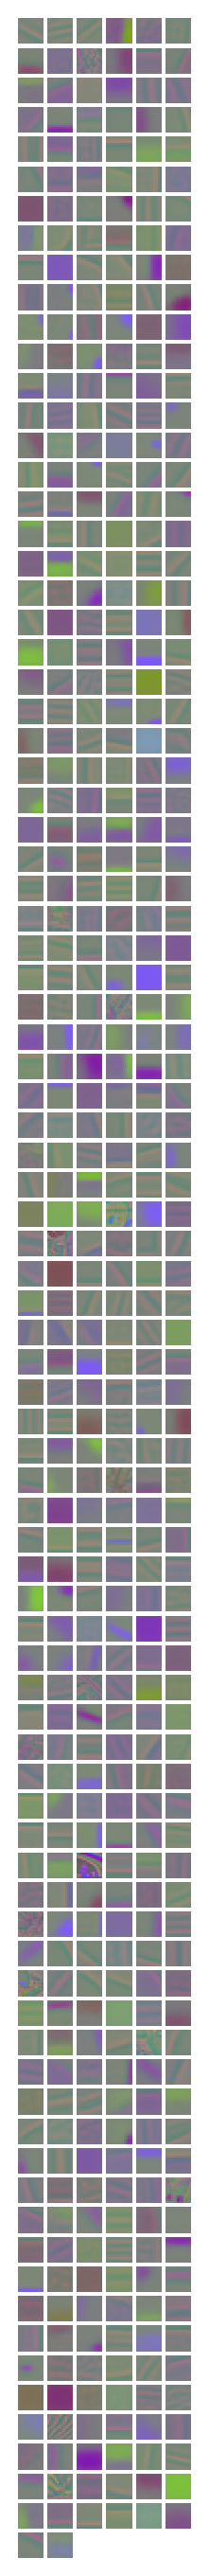
\includegraphics[height=\textheight]{images/centroids}
  \caption{Visualization of the first layer of the best performing model.  The first layer is built by doing convolutional clustering on the unlabelled data.}
\end{figure}

Data augumentation can be performed easily using image module.  We tried multiple types of data augumentation.
\begin{enumerate}
  \item Rotating the image by an angle determined by a gaussian distribution with zero mean and std given by angles ranging from 10 to 20 for various runs.
  \item Scaling/shrinking the image by using image.scale, image.translate and image.crop functions.
\end{enumerate}
The performance of these approaches were at the max on par with the default vgg approach for a maximum of 300 iterations.

\begin{figure}[ht!]
  \centering
  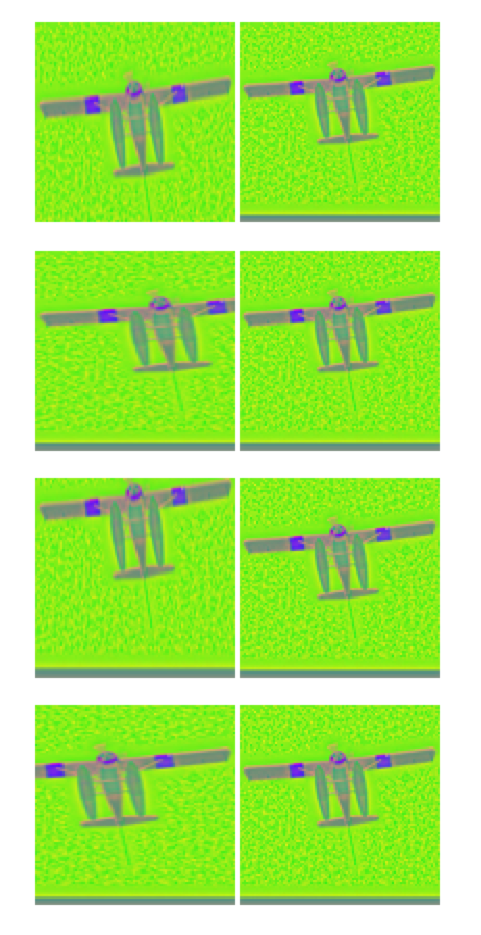
\includegraphics{images/ImageDistortion}
  \caption{Sample distored image.  We distorted the image by using image.scale, image.crop and image.translate and image.rotate.  The values are drawn from a random distribution with zero mean.}
\end{figure}

\section{t-SNE}
T-SNE was built by removing the last layer of the model and propogating randomly drawn 1000 images through the model.  We saved the output of last layer given by a tensor of dimension 1024.  We then followed the tutorial given in the question and got the image by mapping the 1024 dimensional space with the 2D images. The code can be found in tsne.lua and tsne final.ipynb files in\cite{code}.
\begin{figure}[ht!]
  \centering
  \includegraphics[width=0.65\textwidth]{images/tsne}
  \caption{tSNE for 1000 random images.  The clustering is not directly visible in this particular run.  We were unable to run the method again as we were getting segmentation errors in our AWS system.  We were unable to fix the error even after restarting the system, or restarting manifold packages.}
\end{figure}


\section{Kaggle}

\subsection{Experiments}
We tried the following experiments.
\begin{enumerate}
\item Running the base model as it is.  Maximum performance of 68.7\%.
\item Running the base model with minor augumentation such as image rotation and flipping.  Performance of 71.4\%.
\item Running the base model after distorting the image with parameters drawn from gaussian distribution.  This model was highly unpredictable and didn't perform well. 
\item Run kmeans on 13 $\times{}$ 13 patch of images from 10,000 samples and use the centroids as first layer.
\item Run kmeans on 13 $\times{}$ 13 patch of images from 100,000 with 12 patches per image. This gave the maximum performance of 73.5\%.
\end{enumerate}

The results and the performance are as given in the graphs below.

%Kmeans folder
\begin{figure}[ht!]
  \centering
  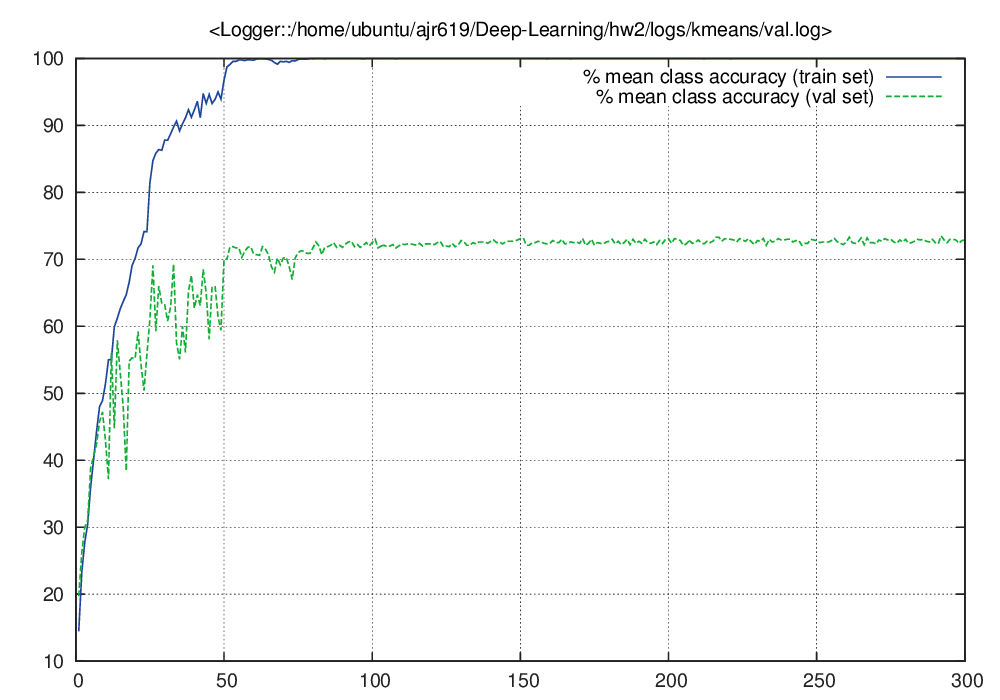
\includegraphics[width=\textwidth]{images/kmeans/val}
  \caption{Epoch vs train/validation accuracy for the best performing model. The best validation accuracy is 73.5\%}
\end{figure}

%Kmeans.1 folder
\begin{figure}[ht!]
  \centering
  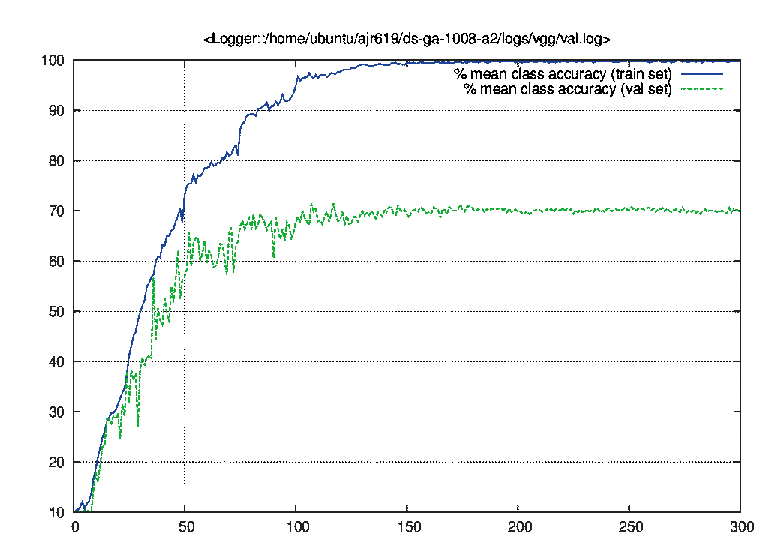
\includegraphics[width=\textwidth]{images/kmeans.1/val}
  \caption{Epoch vs train/validation accuracy for the default vgg model with data augumentation consisting of image flipping/rotation. The best validation accuracy is 71.4\%}
\end{figure}

%vgg folder
\begin{figure}[ht!]
  \centering
  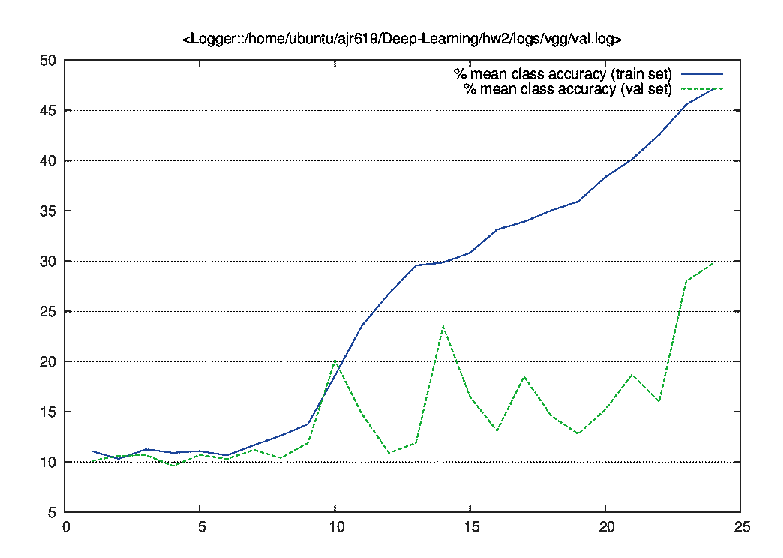
\includegraphics[width=\textwidth]{images/vgg/val}
  \caption{Epoch vs train/validation accuracy.  This model scales and rotates the image to a larger degree than the previous model and thus the performance is highly unpredictable.}
\end{figure}

%vgg folder in path:/home/ubuntu/ajr619/ds-ga-1008-a2/logs
\begin{figure}[ht!]
  \centering
  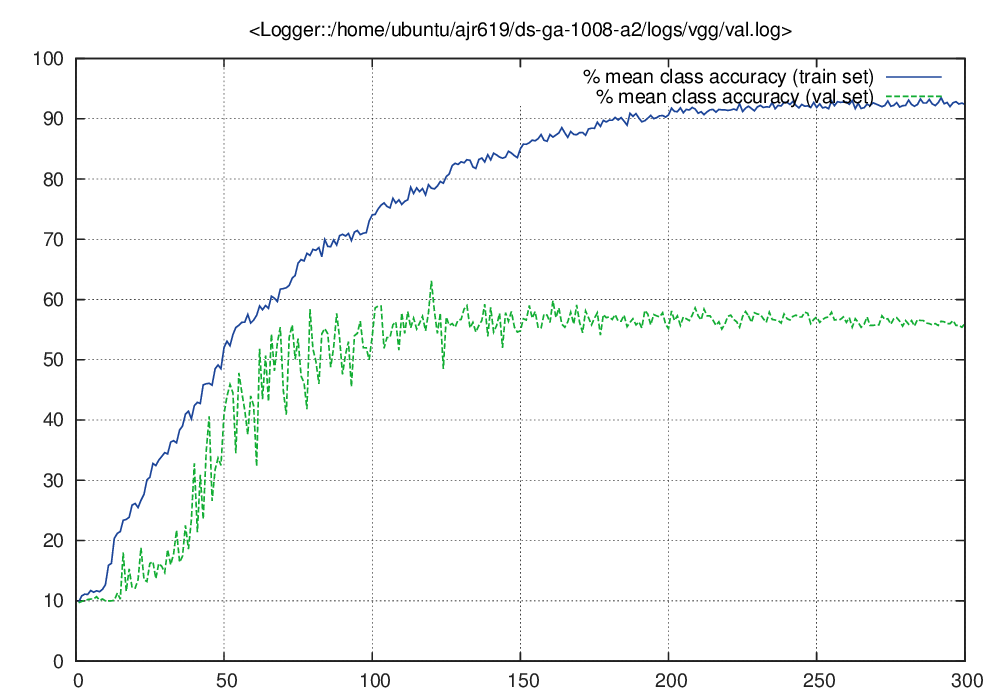
\includegraphics[width=\textwidth]{images/vggInDS-ga/val}
  \caption{Peroformance of model ran with \~3 patch per image for a subset of 10,000 unlabelled images.}
\end{figure}

\begin{thebibliography}{9}
\bibitem{model} \url{https://s3.amazonaws.com/shallowlearners/a2/model.net0.735}
\bibitem{code}\url{gitHub.com/rajegannathan/deep-learning/hw2 as the repository url}
\end{thebibliography}

\end{document}
